\documentclass[a4paper,12pt,onehalfspacing]{report}
\usepackage{graphicx}
\usepackage{subcaption}
\usepackage[export]{adjustbox}
\usepackage{placeins}
\usepackage{titlesec}
\graphicspath{{./Figures/}}
\usepackage{hyperref}
\usepackage{xcolor}
\hypersetup{
    colorlinks,
    linkcolor={red!75!black},
    citecolor={blue!75!black},
    urlcolor={blue!75!black}}
\usepackage[utf8]{inputenc}
\newcommand{\HRule}{\rule{.9\linewidth}{.6pt}}
\usepackage{geometry}
\usepackage{chngcntr}
\counterwithin{table}{section}
\counterwithin{figure}{section}
\usepackage{afterpage}
\usepackage[export]{adjustbox}
\usepackage{datetime}
\usepackage{amsfonts, amsmath, amssymb, mathtools, amsthm, mathrsfs}
\usepackage{cancel}
\usepackage{physics}
\usepackage{cleveref}
% \usepackage{times}

\titleformat{\chapter}[display]
{\normalfont\huge\bfseries\raggedleft}{\thechapter}{10pt}{\Huge}
\AtBeginDocument{\renewcommand{\bibname}{References}}

\tolerance=1
\emergencystretch=\maxdimen
\hyphenpenalty=10000
\hbadness=10000

\newdateformat{monthyeardate}{%
  \monthname[\THEMONTH] \THEYEAR}
\newcommand\emptypage{
    \newpage
    \null
    \thispagestyle{empty}
    % \addtocounter{page}{-1}
    }

\newgeometry{
	% paper=a4paper, % Change to letterpaper for US letter
	inner=1in, % Inner margin
	outer=1in, % Outer margin
	bindingoffset=.5cm, % Binding offset
	top=0.75in, % Top margin
	bottom=0.75in, % Bottom margin
	% showframe, % Uncomment to show how the type block is set on the page
}
\usepackage{setspace}
\setstretch{1.5}
%%%%%%%%%%%%%%%%%%%%%%%%%%%%%%%%%%%%%%%%%%%
%%%%%%%%%%%%%%%% Change %%%%%%%%%%%%%%%%%%
%%%%%%%%%%%%%%%%%%%%%%%%%%%%%%%%%%%%%%%%%%%
\newcommand{\ttitle}{Constraining Dense Matter Equations of State through Non-Radial Oscillation Modes}
\newcommand{\supname}{Dr. Monika Sinha} 
\newcommand{\degree}{Master of Science}
\newcommand{\authorname}{Pratik Thakur}
\newcommand{\rn}{M21PH022}
\newcommand{\univname}{IIT Jodhpur} 
\newcommand{\deptname}{Department of Physics}
%%%%%%%%%%%%%%%%%%%%%%%%%%%%%%%%%%%%%%%%%%%%%%%%

\begin{document}

\begin{titlepage}
    \begin{center}
    \begin{flushright}
    % \Huge{\textbf{{\ttitle}}}
    \Huge{\textbf{\emph{Constraining}\\Dense Matter Equations of State\\\emph{through}\\Non-Radial Oscillation Modes}}
    \end{flushright}
    \vfill
    \begin{flushright}
    \large{\emph{A Project Report Submitted by}}\\
    \huge{\textbf{\authorname}}
    \end{flushright}
    \vfill
    \begin{flushright}
    \large{{\emph{in partial fulfilment of the requirements for the award of the degree of}}}\\
    \huge{\textbf{\degree}}
    \end{flushright}
    \vfill
    
\includegraphics[width=0.3\textwidth,right]{IITJlogo.jpg}
    \begin{flushright}
    \Large{\textbf{Indian Institute of Technology Jodhpur}}\\
    \Large{\textbf{\deptname}}\\
    \Large{\emph{\monthyeardate\today}}
    \end{flushright} 
    \end{center}
\end{titlepage}

\emptypage
\pagenumbering{roman}
\setcounter{page}{2}
\begin{flushright}
    \huge{\chapter*{Declaration}}
\end{flushright}
\addcontentsline{toc}{chapter}{Declaration}
I hereby declare that the work presented in this Project Report titled `\ttitle{}' submitted to the Indian Institute of Technology Jodhpur in partial fulfilment of the requirements for the award of the degree of \degree, is a bonafide record of the research work carried out under the supervision of \supname. The contents of this Project Report in full or in parts, have not been submitted to, and will not be submitted by me to, any other Institute or University in India or abroad for the award of any degree or diploma.
\vspace{1cm}
\begin{flushright} 
    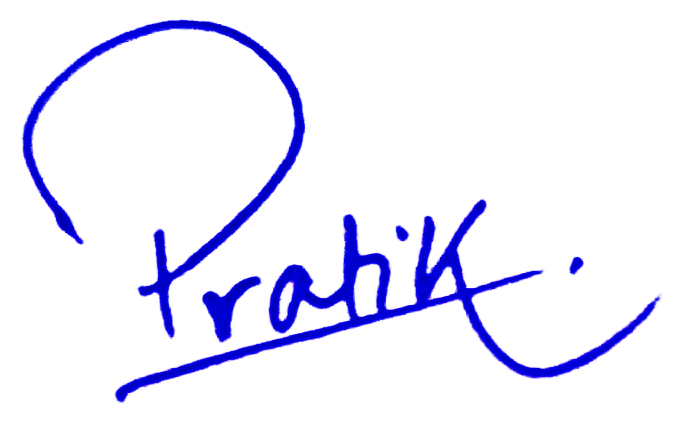
\includegraphics[width=0.15\textwidth,right]{Sign.png}
    \large{\textbf{Signature}}\\
    \emph{\authorname}\\
\rn
\end{flushright}
\emptypage
\begin{flushright}
    \huge{\chapter*{Certificate}}
\end{flushright}
\addcontentsline{toc}{chapter}{Certificate}
This is to certify that the Project Report titled `\ttitle', submitted by \authorname{} (\rn{}) to the Indian Institute of Technology Jodhpur for the award of the degree of \degree{}, is a bonafide record of the research work done by him under my supervision. To the best of my knowledge, the contents of this report, in full or in parts, have not been submitted to any other Institute or University for the award of any degree or diploma.
\vspace{3cm}
\begin{flushright}
\large{\textbf{Signature}}\\
\supname\\
\end{flushright}

\emptypage
\begin{flushright}
    \huge{\chapter*{Acknowledgements}}
\end{flushright}
\addcontentsline{toc}{chapter}{Acknowledgements}
I would like to express my deepest gratitude and appreciation to all those who have contributed to the completion of this Master's thesis.

Firstly, I am indebted to my supervisor, \supname{}, for her invaluable guidance and support throughout this research endeavour. Her mentorship and insightful feedback have been instrumental in shaping the direction and quality of this work. 

I extend my heartfelt thanks to Dr. Vivek B. Thapa and Mr Anil Kumar who willingly shared their time and expertise, making this research possible. Their willingness to engage in discussions, provide valuable insights, and offer assistance has been pivotal in enhancing the depth and validity of my thesis. This work would not have been possible without their constant support.

Finally, I am indebted to my friends Manoj and Ayanava for the long walks and endless discussions (most of them in Bangla, some in a British accent), and to Harshita for her constant love and motivation throughout my studies. I am grateful to my parents, Mr Prantik Thakur and Mrs Rumpa Thakur, and my brother Praneet for their love and unwavering support. I wouldn't be who I am without them.

\emptypage
\begin{flushright}
    \huge{\chapter*{Abstract}}
\end{flushright}
\addcontentsline{toc}{chapter}{Abstract}
Due to their extremely dense interiors, neutron stars provide a means to study properties of matter with densities beyond the nuclear saturation density. Due to the immense difficulty of reproducing these extreme conditions in the laboratory, probing neutron star matter has to be done via theoretically constructed equations of state, which are then constrained by observational data. In this work, we consider $\beta-$equlibrated cold neutron stars, finite temperature proto-neutron stars, hybrid stars with a hadron-quark phase transition, and the presence of exotic particles or dark matter in compact objects, and explore how non-radial, quasinormal fluid oscillation modes can be used to constrain dense matter equations of state. We also derive the equations governing the structure of spherically symmetric relativistic stars, and the non-radial oscillation modes. Finally, we also see the effects of various equations of state on the mass-radius relation, and the dimensionless tidal deformability of the stars, and make a qualitative observation about how these oscillation mode frequencies are dependent on the equation of state parameters.

\emptypage
\begin{flushright}
    \huge{\chapter*{List of Publications}}
\end{flushright}
\addcontentsline{toc}{chapter}{List of Publications}
This thesis is based on the following article: 

\begin{enumerate}
    \item Vivek B. Thapa, Mikhail V. Beznogov, Adriana R. Raduta, and \textbf{Pratik Thakur}. “Frequencies of $f$- and $p$-Oscillation Modes in Cold and Hot Compact Stars.” arXiv, February 22, 2023. http://arxiv.org/abs/2302.11469.\\ (In production stage)
\end{enumerate}

And several more works in progress.

\emptypage
\begin{flushright}
\tableofcontents
% \clearpage
\listoffigures
\listoftables
\end{flushright}

\newpage
\emptypage
\chapter{Introduction}
\pagenumbering{arabic}

Neutron stars, characterized by their remarkable compactness and strong gravitational forces, rely on the degeneracy pressure of neutrons to support themselves. A lack of experimental data about the interior of these stars, as well as our current inability to attain such high densities in our laboratories has made neutron stars one of the most important candidates to study dense matter physics. To model the neutron stars, we often start by constructing a Lagrangian, taking into effect the interactions presumed to be happening in the star, and using this, get an equation of state which describes how pressure varies with energy density. Equations of state can also be constructed by randomising a variable such as the speed of sound in the star, and putting constraints on the generated equations of state from theory and observation. The study of neutron star interiors is then an exercise in finding constraints on the properties of the neutron stars and the microscopic interactions in consideration, all of which follow from the equation of state. 

\section{Non-Radial Modes} \label{sec: non rad modes}

Non-radial oscillation modes in relativistic stars are a fundamental aspect of the theory of stellar oscillations. These modes correspond to deformations of the star's shape and structure, as opposed to radial modes, which correspond to changes in the star's radius. The non-radial oscillation modes can be classified into different families based on their angular dependence and their restoring forces, viz. the fluid, $f-$ (fundamental), $p-$ (pressure) and $g-$ (gravity) modes, $r-$ (rotational) modes, $i-$ (inertial) modes, $w-$ spacetime modes etc. \cite{kokkotasQuasiNormalModesStars1999,cowlingNonradialOscillationsPolytropic1941}. Several of these modes
can be excited during supernovae explosions or in an isolated perturbed compact star as in the post-merger phase of binary compact stars \cite{kokkotasInverseProblemPulsating2001,stergioulasGravitationalWavesNonaxisymmetric2011,PhysRevD.101.084039}. Even during the inspiral phase of compact stars, the $f-$mode may be excited \cite{chirentiGravitationalWavesFmodes2017,PhysRevResearch.3.033129}. Due to their extreme sensitivity to the interior compositions of these compact objects, these quasi-normal modes can provide great insight into constraining the dense matter equations of state \cite{sathyaprakashPhysicsAstrophysicsCosmology2009}. Many works \cite{anderssonGravitationalWavesPulsating1996,anderssonGravitationalWaveAsteroseismology1998,kokkotasInverseProblemPulsating2001} have been accomplished to understand the implications of EoS on quasi-normal modes. For example, it has been concluded in past literature \cite{sotaniDensityDiscontinuityNeutron2001,Sotani,vasquezfloresDiscriminatingHadronicQuark2014} that the $g-$modes may be able to imply the existence of phase transition in the star, due to their sensitivity to density discontinuities. 

The motivation to study these modes comes from the possibility of observing them. With enhanced next-generation telescopes such as the Einstein Telescope and Cosmic Explorer, having sensitivities that are ten-fold in comparison to present instruments, we expect to be able to detect some of these fluid modes. Quadrupolar oscillations (l=2) of all modes lead to the emission of GWs. With the advent of enhanced
next-generation telescopes like the Cosmic Explorer and the Einstein telescope, which carry about 10 times the sensitivity of Advanced LIGO, the possibility of detection of these modes increase \cite{kokkotasInverseProblemPulsating2001,Zhao_universal_f_g}.

In general relativity, the oscillation modes of a star are described by perturbations to the background spacetime metric, which is governed by a set of partial differential equations known as the Regge-Wheeler-Zerilli equations. Coupled with the perturbations of the stellar fluids, the complete set of differential equations governing these non-radial oscillations were first derived in the seminal work by Thorne and Campolattaro \cite{Thorne_Campo}. These equations give the frequency and damping time of the non-radial modes. However, due to the complexity of these equations, McDermott introduced the relativistic Cowling approximation \cite{mcdermottNonradialGmodeOscillations1983}, wherein the perturbations of the spacetime metric was neglected, in line with the approximation made by Cowling to neglect the perturbations of the gravitational potential, when he was studying non-radial modes in Newtonian gravity \cite{cowlingNonradialOscillationsPolytropic1941}.

In this work, we'll restrict our study to non-radial fluid oscillation modes, primarily the $f-$, $p-$ and $g-$ modes within the relativistic Cowling approximation. 

\section{On Equations of State}\label{sec: eos intro}

We'll now briefly describe the motivation for the equations of state considered in this work. Aside from the pure nuclear equations of state, due to recent astrophysical observations of massive neutron stars, there is growing interest in exploring the possibility of exotic matter within their interiors. Although neutrons are believed to be the primary constituents of these stellar objects, due to the extreme conditions, it is expected that a mixture of other baryons and exotic particles also exists within them. These findings have sparked further investigations into the nature and properties of this exotic matter, providing valuable insights into the fundamental physics at play in these extreme environments. 

By far most of the works on oscillation mode frequencies have been accomplished considering the zero temperature equations of state. But as mentioned in \cite{ferrariGravitationalWavesNewly2003}, proto-neutron stars have been considered as potential gravitational wave sources by terrestrial detectors such as LIGO and Virgo. The temperature of such stars may reach up to $\sim 50 MeV$ \cite{dexheimerProtoNeutronNeutron2008}. Moreover, proto-neutron stars have been found to show the same quasinormal oscillation modes as cold stars \cite{ferrariGravitationalWavesNewly2003,burgioOscillationsHotYoung2011,PhysRevD.94.044043,PhysRevD.100.083008}. So in order to appropriately understand the oscillation modes, one needs to take into account the thermal effects on the dense matter equation of state. 

Finally, we wish to consider non-radial modes in dark matter admixed compact objects. There is conclusive evidence from cosmological and astrophysical observations of rotation curves of individual galaxies, galaxy clusters, and anisotropic microwave background that the dominant contribution to the matter density in the universe is in the form of `dark matter' which interacts very weakly with ordinary matter \cite{bertoneParticleDarkMatter2005}. However, the gravitational effects of dark matter are not insignificant. Since as of yet, there is no evidence of beyond standard model interactions between dark matter and standard model particles, and in hindsight that the interaction strength, if any, would be extremely weak, it is not far-fetched to assume that dark matter interacts with ordinary matter purely gravitationally. Due to the extreme nature of neutron stars which allows them to accrete matter, and considering the amount of dark matter in the universe, there is a likelihood that dark matter may be accreted inside stars. This is also motivated by the tension between nuclear physics and astrophysical observations- neutron star models with ordinary matter tend to support high maximum masses and high tidal deformability, while observational data suggest that neutron stars are massive, but not very deformable \cite{ciancarellaConstrainingMirrorDark2021}. The inclusion of dark matter in neutron stars can act to alleviate these opposing observations. 

\emph{Throughout this work, we'll consider all quantities in units of $\hbar=c=G=1$, and follow the spacetime invariant convention of $\dd s^2= -\dd t^2+ \dd x^2+ \dd y^2+ \dd z^2$}

\emptypage
\chapter{Stellar Structure Equations}

Since we will be studying non-radial modes in neutron stars, the primary goal will of course be to construct the star itself. Given the immense compactness of neutron stars, general relativistic effects cannot be neglected and must be taken into consideration while constructing the star. Although these equations are present in every textbook of general relativity, it is useful to rederive them because as we will see, using some analysis, we can then directly quote the modifications required for two-fluid stars. We will be considering non-rotating spherically symmetric stars composed of a perfect fluid.

\section{Components of the Einstein Tensor}

The Einstein field equations are $G_{\mu \nu }=8\pi T_{\mu \nu }$ with the various terms being \cite{MTW_GR}
\begin{align*}
    \text{Einstein Tensor}&:& G_{\mu \nu }&=R_{\mu \nu }-\frac{R g_{\mu \nu }}{2}\\[5pt]
    \text{Ricci Tensor}&:& R_{\mu \sigma }&=R^{\lambda }{}_{\mu \lambda \sigma }\\[5pt]
    \text{Ricci Scalar}&:& R&= R^\lambda{}_\lambda\\[5pt]
    \text{Riemann Curvature Tensor}&:& R^{\lambda }{}_{\mu \nu \sigma }&=\Gamma ^{\lambda }{}_{\mu \sigma ,\nu }- \Gamma ^{\lambda }{}_{\mu \nu ,\sigma }+\Gamma ^{\rho }{}_{\mu \sigma } \Gamma ^{\lambda }{}_{\nu \rho }- \Gamma ^{\rho }{}_{\mu \nu } \Gamma ^{\lambda }{}_{\sigma \rho }\\[5pt]
    \text{Christoffel Symbols}&:& \Gamma ^{\lambda }_{\mu \nu }&=\frac{1}{2} g^{\lambda \rho }\left(\frac{\partial g_{\nu \rho }}{\partial \mu }-\frac{\partial g_{\mu \nu }}{\partial \rho }+\frac{\partial g_{\rho \mu }}{\partial \nu }\right)\\[5pt]
    \text{Energy-momentum Tensor}&:& T_{\mu\nu}
\end{align*}

Here $g_{\mu\nu}$ is the spacetime metric. The most general spherically symmetric line element that can be constructed is: \cite{MTW_GR}
\begin{equation}
    ds^2= - e^{2\Phi}\ dt^2+  e^{2\Lambda}\ dr^2+r^2\ d\theta^2+r^2\sin^2\theta\ d\phi^2\label{eq: ds2}
\end{equation}
With the corresponding metric being

\begin{align}
    g_{\mu\nu}= \begin{bmatrix}
        - e^{2\Phi} & 0 & 0 & 0 \\
        0 &  e^{2\Lambda} & 0 & 0 \\
        0 & 0 & r^2 & 0 \\
        0 & 0 & 0 & r^2\sin^2\theta \\
    \end{bmatrix}\qquad  
    g^{\mu\nu}= \begin{bmatrix}
        - e^{-2\Phi} & 0 & 0 & 0 \\
        0 &  e^{-2\Lambda} & 0 & 0 \\
        0 & 0 & \frac{1}{r^2} & 0 \\
        0 & 0 & 0 & \frac{1}{r^2\sin^2\theta} \\
    \end{bmatrix}\label{eq: metric}
\end{align}

Since we're considering static stars, the variables $\Phi$ and $\Lambda$ are functions of the radius $r$ alone. Now we calculate all the components of the Einstein field equations for the metric defined above. The non-trivial ones are given in \cref{table: symbols} (where $'$ represents a derivative with respect to the radius $r$): 

\begin{table}[ht!]
    \centering
    \begin{tabular}{ |c|c|c| }
    \hline
    &&\\[0.01ex]
    Type & Symbol & Value \\[0.01ex]
    &&\\[0.01ex]
    \hline\hline
    &&\\[1ex]
    Christoffel Symbols & $ \Gamma ^{t}_{tr},\  \Gamma ^{t}_{rt}$ & $\Phi '$  \\[1.5ex]
    & $\Gamma ^r_{tt}$ & $e^{2 \Phi-2 \Lambda} \Phi '$ \\[1.5ex]
    &$\Gamma ^r_{rr}$ & $\Lambda '$\\[1.5ex]
    &$\Gamma ^r_{\theta \theta}$ & $-re^{-2 \Lambda}$\\[1.5ex]
    &$\Gamma ^r_{\phi\phi}$ & $-re^{-2 \Lambda} \sin ^2\theta$\\[1.5ex]
    &$\Gamma ^{\theta}_{r\theta},\ \Gamma ^{\theta}_{\theta r},\ \Gamma ^{\phi }_{r\phi },\  \Gamma ^{\phi }_{\phi r}$ & $\frac{1}{r}$\\[1.5ex]
    &$\Gamma ^{\theta }_{\phi\phi }$& $-\sin \theta \cos \theta$\\[1.5ex]
    &$\Gamma ^{\phi }_{\theta\phi },\  \Gamma ^{\phi }_{\phi \theta}$ & $\cot \theta$\\[2ex]
    \hline
    &&\\[1ex]
    Ricci Tensor & $R_{tt}$ & $e^{2 \Phi-2 \Lambda} \qty(\Phi ''+\Phi '^2-  \Lambda '\Phi ' +\frac{2\Phi '}{r})$\\[3ex]
    & $R_{rr}$ & $e^{-2 \Phi+2 \Lambda}R_{tt}+ \frac{2}{r}\qty(\Lambda'+ \Phi ')$\\[3ex]
    &$R_{\theta \theta }$ & $e^{-2 \Lambda } \qty(e^{2 \Lambda }+r \Lambda'-r \Phi'-1)$\\[3ex]
    &$R_{\phi \phi }$ & $R_{\theta\theta }\sin ^2\theta$\\[2ex]
    \hline
    &&\\[1ex]
    Einstein Tensor &$G_{tt}$ & $\frac{e^{2 \Phi-2 \Lambda}}{r^2}\qty(2 r \Lambda '+e^{2 \Lambda}-1)$\\[3ex]
    &$G_{rr}$ & $\frac{1}{r^2}\qty(2 r \Phi '-{e^{2 \Lambda}+1})$\\[3ex]
    &$G_{\theta \theta }$ & $r e^{-2 \Lambda } \qty(r \Phi ''+r \Phi '^2 +\Phi'-\Lambda'-r \Lambda ' \Phi ')$\\[3ex]
    &$G_{\phi \phi }$ & $G_{\theta \theta }\sin ^2\theta$\\[2ex]
    \hline
    \end{tabular}
    \caption{Various components of the Einstein field equations for the general spherically symmetric metric}
    \label{table: symbols} % is used to refer to the table in the text
\end{table}

\section{Energy Momentum Tensor of a Perfect Fluid}

The energy-momentum tensor of a perfect fluid in general relativity is given by
\begin{equation}
    T^{\mu\nu}= (p+\varepsilon)U^{\mu} U^{\nu}+ pg^{\mu\nu}\label{eq: perfect fluid}
\end{equation}
with $U^\mu$ being the four velocity, $p$ the pressure and $\varepsilon$ the energy density. Since we're considering a static star, the spatial components of the four-velocity are 0. The temporal component is given by the four-velocity normalization condition: 
\begin{eqnarray*}
    g_{\mu\nu} U^\mu U^\nu &=& -1 \\
    - e^{2\Phi}U^0 U^0 &=& -1\\ 
    U^0 &=&  e^{-\Phi}
\end{eqnarray*}
Hence the four-velocity for a static fluid in the general spherically symmetric line element is: 
\begin{equation}
    U^\mu= [ e^{-\Phi}, 0, 0, 0]\qquad U_\mu= [- e^{\Phi}, 0, 0, 0]\label{eq: four velocity}
\end{equation}
And the energy-momentum tensor is: 
\begin{align}
    T_{\mu\nu}= \begin{bmatrix}
         e^{2\Phi}\varepsilon & 0 & 0 & 0 \\
        0 &  e^{2\Lambda}p & 0 & 0 \\
        0 & 0 & r^2p & 0 \\
        0 & 0 & 0 & r^2p\sin^2\theta
    \end{bmatrix}\label{eq: perfect fluid elements}
\end{align}
The conservation of energy-momentum implies $T^{\mu\nu}{}_{;\nu}=0$, where `$;$' represents the covariant derivative. Thus
\begin{align*}
    0 &= \left[(p+\varepsilon)U^{\mu} U^{\nu}+ pg^{\mu\nu}\right]_{;\nu}\\
    0 &= (p+\varepsilon)_{;\nu}U^\mu U^\nu+ (p+\varepsilon)[U^\mu{}_{;\nu} U^\nu + U^\mu U^\nu{}_{;\nu}] + p_{;\nu}g^{\mu\nu}
\end{align*}

Moreover, since $g^{\mu\nu}_{\ \ \ ;\nu}= 0$ then: 
\begin{align}
    0&= [U^\mu U_\mu]_{;\nu}= U^\mu_{\ ;\nu}U_\mu + U_{\mu;\nu}U^\mu\nonumber\\
    0&=U^\mu_{\ ;\nu}U_\mu + [g_{\alpha\mu}U^\alpha]_{;\nu}[g^{\beta\mu}U_\beta]\nonumber\\
    0&=U^\mu_{\ ;\nu}U_\mu + U^\alpha_{\ ;\nu}U_\alpha\nonumber\\
    \therefore 0&= U^\mu_{\ ;\nu}U_\mu= U^\mu U_{\mu;\nu} \label{eq: U contraction}
\end{align}
We now want to extract the momentum conservation law, for which we need to take a projection on the spacelike components of the energy-momentum conservation law. This is done by contracting $T^{\mu\nu}{}_{;\nu}=0$ with $h_{\mu\lambda}= g_{\mu\lambda}+U_{\mu}U_\lambda$ and using \cref{eq: U contraction}:
\begin{align*}
    0 =&\ (p+\varepsilon)_{;\nu}[g_{\mu\lambda}U^\mu U^\nu+U_{\mu}U_\lambda U^\mu U^\nu]+(p+\varepsilon)[U^\mu_{\ ;\nu} U^\nu g_{\mu\lambda} + U^\mu U^\nu_{\ ;\nu}g_{\mu\lambda}] \\
    &+(p+\varepsilon)[U^\mu_{\ ;\nu} U^\nu U_{\mu}U_\lambda + U^\mu U^\nu_{\ ;\nu}U_{\mu}U_\lambda]+ p_{;\nu}g^{\mu\nu}[g_{\mu\lambda}+U_{\mu}U_\lambda]\\
    0 =&\ (p+\varepsilon)_{;\nu}[U_\lambda U^\nu-U_\lambda U^\nu]+(p+\varepsilon)[U^\mu_{\ ;\nu} U^\nu g_{\mu\lambda} + U_\lambda U^\nu_{\ ;\nu}] \\
    &+(p+\varepsilon)[0\cdot U^\nu U_\lambda - U^\nu_{\ ;\nu}U_\lambda]+ p_{;\nu}[\delta^\nu_\lambda+U^{\nu}U_\lambda]\\
    0 =&\ (p+\varepsilon)U_{\lambda;\nu} U^\nu + p_{;\lambda}+p_{;\nu}U^{\nu}U_\lambda
\end{align*}
Replacing $\lambda$ by $\mu$, and expanding the covariant derivative, we get the \emph{relativistic Euler equation}
\begin{equation}
    (p+\varepsilon)U^\nu\partial_\nu U_\mu -(p+\varepsilon)U^\nu \Gamma^{\alpha}_{\sigma\nu}U_\alpha = -\partial_\mu p- U_\mu U^\nu \partial_\nu p \label{eq: relativistic Euler}
\end{equation}

For the four-velocity of a static fluid (\cref{eq: four velocity}), and taking the free index in \cref{eq: relativistic Euler} to be $\mu=r$, the relativistic Euler equation reduces to :
\begin{align*}
    (p+\varepsilon)U^\nu\partial_\nu U_r -(p+\varepsilon)U^\nu \Gamma^{\alpha}_{\sigma\nu}U_\alpha &= -\partial_r p- U_r U^\nu \partial_\nu p\\
    -(p+\varepsilon)U^t \Gamma^{t}_{\sigma t}U_t &= -\partial_r p
\end{align*}
From \cref{table: symbols}, we see that the above is non-zero only for $\sigma= r$ with $\Gamma^{t}_{r t}= \Phi'$. Substituting this in the above equation and using $U^t= e^{-\Phi}$, we get the radial variation of the pressure in a star as:
\begin{equation}
    \dv{p}{r}= -(p+\varepsilon)\dv{\Phi}{r} \label{eq: dp_dr}
\end{equation}


\section{Exterior Solution}

Far away from the spherically symmetric source, our metric must reduce to the Minkowskian metric. Since at that point, the energy-momentum tensor is identically 0, the Einstein field equations are equivalent to $G_{\mu\nu}= 0 \Rightarrow R_{\mu\nu}= 0$. From the Ricci tensor components, we thus get: 
\begin{align*}
    \text{R}_{rr}&= e^{-2 \Phi+2 \Lambda}\text{R}_{tt}+ \frac{2}{r}\left(\Lambda'+ \Phi '\right)\\
    0 &= 0+ \frac{2}{r}\left(\Lambda'+ \Phi '\right)\\
    \Phi' &= -\Lambda'\\
    \therefore \Phi &= -\Lambda + k
\end{align*}

Where $k$ is some arbitrary constant. However, if we plug $\Phi$ into the line element (\cref{eq: ds2}),the $dt^2$ component becomes $-e^{2k}e^{-2\Lambda}dt^2$. We can now make a coordinate transformation $dt' \rightarrow e^k dt$, which will take away the constant factor, and thus, in general, we can set $k=0$ to get: $\Phi= -\Lambda$ at $r$ much greater than the radius of the star. Now setting $R_{\theta \theta }= 0$ we get: 
\begin{align}
    \text{R}_{\theta \theta }&=e^{-2 \Lambda } \qty(e^{2 \Lambda }+r \Lambda '-r \Phi '-1)= 0\nonumber\\
    e^{-2\Phi }-2r \Phi '-1&=0\nonumber\\
    (re^{2\Phi})'&=1\nonumber\\
    \Phi &= \frac{1}{2}\ln\left[{1+\frac{k}{r}}\right]\label{eq: Phi_step}
\end{align}

The line element thus becomes: 
\begin{align*}
    ds^2 &= -\mathrm{e}^{2\Phi}\ dt^2+ \mathrm{e}^{-2\Phi}\ dr^2+r^2\ d\theta^2+r^2\sin^2\theta\ d\phi^2\\
    ds^2 &= -\left[1+\frac{k}{r}\right]\ dt^2+ \left[1+\frac{k}{r}\right]^{-1}\ dr^2+r^2\ d\Omega^2
\end{align*}

In the Newtonian limit, particle velocities are slow such that $\frac{dx}{d\tau}\ll \frac{dt}{d\tau}$ and the geodesic equation \cite{Weinberg} reduces to $\ddot{x}^\mu + \Gamma^{\mu}_{\alpha\beta}\ \dot{x}^\alpha\dot{x}^\beta=0\rightarrow \ddot{x}^\mu + \Gamma^{\mu}_{tt}\ (\dot{x}^t)^2= 0 $

Taking the free index to be $\mu= r$, and using $\Gamma ^r_{tt} = e^{2 \Phi-2 \Lambda} \Phi '$ and \cref{eq: Phi_step}, the geodesic equation becomes
\begin{align*}
    0&= \frac{\dd^2 r}{\dd\tau^2}+ e^{4\Phi} \Phi'\left(\frac{\dd t}{\dd\tau}\right)^2 \\[1.5ex]
    \frac{\dd^2 r}{\dd\tau^2}&= \frac{k}{2r^2}\qty(1+\frac{k}{r})\\[1.5ex]
    \frac{\dd^2 r}{\dd\tau^2}&\approx \frac{k}{2r^2}\qquad \qty{r\rightarrow \infty}
\end{align*}

But in the Newtonian limit, $\frac{\dd^2 r}{\dd\tau^2}= \frac{-M}{r^2}$. Thus $\frac{k}{2r^2}= \frac{-M}{r^2}\Rightarrow k=-2M$ (in units of G=1), where $M$ is the mass of the star. Hence the exterior solution to our line element is the Schwarzschild solution: 
\begin{equation}
    \dd s^2 = -\qty(1+\frac{2M}{r})\ \dd t^2+ \qty(1+\frac{2M}{r})^{-1}\ \dd r^2+r^2\ \dd\Omega^2\\
\end{equation}
And the metric function $\Phi$ is $\Phi= -\Lambda= \frac{1}{2}\ln\qty({1-\frac{2M}{r}})$ at a point $r$ greater than the radius of the star. 

\section{Interior Solution}

To find the form of the metric inside the star, we have to solve the Einstein field equations. We use \cref{table: symbols,eq: perfect fluid elements} form which the temporal component of the field equations are:
\begin{align*}
    G_{tt}&= 8\pi T_{tt}\\
    \frac{e^{2 \Phi-2 \Lambda}}{r^2}\qty(2 r \Lambda '+e^{2 \Lambda}-1)&= 8\pi\mathrm{e}^{2\Phi}\varepsilon\\
    2 r \Lambda 'e^{-2 \Lambda }-e^{-2 \Lambda }+1&= 8\pi\varepsilon r^2\\
    \qty[r\qty(1-e^{2 \Lambda})]'&= 8\pi\varepsilon r^2
\end{align*}
To match expressions with the exterior solution, let's define $\Lambda= -\frac{1}{2}\ln\qty({1-\frac{2M}{r}})$ from which $e^{-2\Lambda}= 1- \frac{2m}{r}$. Then,
\begin{align}
    m' &= 4\pi\varepsilon r^2\label{eq: dm}
\end{align}

Here $m(r)$ is the gravitational mass of the star contained up to radius $r$. 
Now looking at the $G_{rr}$ component, 
\begin{align}
    {G}_{rr} &= 8\pi T_{rr}\nonumber\\
    \frac{1}{r^2}\qty(2 r \Phi '-{e^{2 \Lambda}+1})&= 8\pi e^{2\Lambda}p\nonumber\\
    \Phi '(r)&=\frac{\qty(1-\frac{2m}{r})^{-1}\qty[1+8 \pi p r^2]-1}{2 r}\nonumber\\
    \Phi'(r) &=\frac{m+4 \pi r^3p}{r (r- 2 m)}\label{eq: dPhi}
\end{align}
This equation gives us the variation of $\Phi$ with the radius $r$. Using \cref{eq: dp_dr} we get:
\begin{align}
    p'(r) =-(p+\varepsilon)\qty[\frac{m+4 \pi r^3p}{r (r- 2 m)}]\label{eq: dp}
\end{align}
This is the Tolman-Oppenheimer-Volkov (TOV) equation. The \cref{eq: dm,eq: dp,eq: dPhi} are a set of coupled ordinary differential equations which, upon solving give the structure of the star as well as the metric functions $\Lambda$ and $\Phi$. The boundary conditions are obvious. At the centre of the star, the mass is $0$. The central energy density ($\varepsilon_c$) is an input and the corresponding central pressure ($p_c$) is obtained from the equation of state in consideration. At the surface, the pressure must vanish. Since $\Phi$ must be continuous across the surface of the star, $\Phi$ just outside the star must be equal to the exterior solution of $\Phi$ at that point. The stellar structure equations of general relativity, along with the boundary conditions are thus:
\begin{equation}
    \begin{aligned}
        \dv{m(r)}{r}&= 4\pi r^2 \varepsilon(r) \qquad& m(0) &= 0 \\[2ex]
        \dv{\Phi(r)}{r} &= \frac{m(r)+4 \pi r^3p(r)}{r (r- 2 m(r))} \qquad& \Phi(r=R_*)&= \frac{1}{2}\ln\qty(1-\frac{2M}{R_*})\\[2ex]
        \dv{p(r)}{r}&= -(p(r)+\varepsilon(r))\dv{\Phi(r)}{r} \qquad& p(0)&=p_c;\ \ p(r=R_*)= 0
    \end{aligned}\label{eq: structure eqns}
\end{equation}
Here $M$ is the mass of the star and $R_*$ its radius. Additionally, the metric function $\Lambda$ is given by $$\Lambda(r) = -\frac{1}{2}\ln\qty(1-\frac{2m(r)}{r})$$

\section{Structure Equations in the Two-Fluid Scenario}

To study dark matter admixed stars, these structure equations need to be modified. Let the matter be composed of two perfect fluids labelled `1' and `2'. In general, the total energy density will be $\varepsilon= \varepsilon_1+\varepsilon_2+\varepsilon_{interaction}$. However, if we assume that the two fluids interact purely gravitationally and that there are no, or negligible microscopic interactions between the two fluids, then the interaction term can be dropped. As mentioned in \cref{sec: eos intro}, this is a feasible assumption if one of the two fluids is dark matter. Hence the total energy density and pressure can be separated into individual contributions from the two fluids:
\begin{equation}
        \varepsilon(r)= \varepsilon_1(r)+\varepsilon_2(r);\qquad p(r)= p_1(r)+p_2(r)
\end{equation}
The total mass of the star can thus also be separated into contributions from individual fluids and the changes in the mass equation in \cref{eq: structure eqns} is thus obvious. 
\[\dv{m}{r}=4\pi r^2 \varepsilon\to\dv{m_1+m_2}{r}=4\pi r^2 \qty(\varepsilon_1+\varepsilon_2)\]
The same equation will now hold for each fluid separately. In the $\Phi$ equation, $m$ and $p$ will be replaced by the total mass and total pressure. The pressure equation comes from the conservation of energy-momentum, which must be valid for both fluids individually. Hence the modifications in the structure equations are: 
\begin{equation}
    \begin{aligned}
        \dv{m_i(r)}{r}&= 4\pi r^2 \varepsilon_i(r)\\[2ex]
        \dv{\Phi(r)}{r} &= \frac{[m_1(r)+m_2(r)]+4 \pi r^3[p_1(r)+p_2(r)]}{r \qty(r- 2 [m_1(r)+m_2(r)])}\\[2ex]
        \dv{p_i(r)}{r}&= -(p_i(r)+\varepsilon_i(r))\dv{\Phi(r)}{r}
    \end{aligned}\label{eq: structure eqns twof}
\end{equation}
Here $i=1,2$ labels the fluids. The three ordinary differential equations become five in the two-fluid case. The inputs are now the central energy densities and pressures of both fluids. The radius at which the pressure of a fluid becomes $0$ marks the boundary of that fluid. The total mass of the star is the sum of individual masses of the fluids and is obtained when both the fluid pressures become $0$. 

\section{A Note on Units and the Numerical Algorithm}

For the numerical integration of differential equations, it's always best to work with dimensionless quantities. However, one can get around the need to change variables as long one knows the conversion factors between various units. In the units of $\hbar=c=G=1$, the dimensions of mass and length are the same. Various useful conversions are outlined below. 
For the equation of state, the energy density and pressure are both taken to be in units of $MeV/fm^3$. The units $g/cm^3$ for energy density and $dyne/cm^2$ for pressure is another popular way to tabulate the equation of state and the conversion factors are \cite{Glendenning}:
\begin{align*}
    1\ MeV/fm^3 &= 1.7827\times 10^{12}\ g/cm^3\\
    &= 1.6022\times 10^{33}\ dyne/cm^2
\end{align*}
To solve the structure equations, it's convenient to further convert these quantities to some power of length since these are the dimensions of mass and radius. We have \cite{Glendenning}:
\begin{align*}
    1\  g/cm^3&= 7.4237 \times 10^{-19}\  /km^2\\
    1\  dyne/cm^2 &= 8.2601 \times 10^{-40}\  /km^2
\end{align*}
From which we obtain the conversion from $MeV/fm^3$ to $/Mm^2$ (where $Mm$ is Megameters) as $1\  MeV/fm^3= 1.323423\ /Mm^2$. Upon solving the structure equations, we'll obtain the radius in $Mm$, which we can easily convert to $km$ ($1\ Mm= 1000\ km$) and the mass in $Mm$ can be converted to Solar mass using \cite{Glendenning} $1\ M_\odot = 1.4766\  km$. 

To solve the single fluid-structure equations, \cref{eq: structure eqns}, we employ a Runge-Kutta-4 (RK-4) algorithm, subject to the initial conditions specified. The integration is stopped when the pressure reaches the specified tolerance limit and the values of $r$ and $m$ at this point correspond to the total mass and radius of the star. At this point, the values of $\Phi$ are renormalised to match the boundary condition at the surface. Different central energy densities correspond to unique solutions to the structure equations for a given equation of state. 

For the two-fluid scenario, we're more interested in finding stars with a constant dark matter mass fraction. This fraction is defined as the mass of dark matter divided by the total mass of the star. Since these masses cannot be known until after the structure equations have been solved, then for a certain central energy density of normal matter, a Newton-Raphson root-finding algorithm is employed to find the central energy density of dark matter which will produce the required mass fraction. At some point during the integration of \cref{eq: structure eqns twof}, the pressure of one of the fluids will vanish. This will mark the radius and mass of that particular fluid. At this point, the integration is switched to the single fluid-structure equations, \cref{eq: structure eqns}. When the pressure of the other fluid vanishes as well, the integration is stopped. There can be two situations if one of the fluids is dark matter: If the dark matter pressure reaches $0$ first, then the star has dark matter concentrated in the interior, forming a dark matter core. If however, the pressure of normal matter vanishes first, then the dark matter extends outside the star, forming a dark matter halo. The mass of the star is going to be the sum of the masses of the dark and normal matter. However, constraints on the radius of the stars obtained via X-ray or radio measurements cannot detect a dark matter halo and in these cases, the radius of the star must be taken to be the radius of the normal matter.

\chapter{Non-Radial Oscillation Modes}

As mentioned in \cref{sec: non rad modes}, our main focus in this work will be to study the fluid oscillation modes within the relativistic Cowling approximation for the dominant $l=2$ mode. The study of non-radial oscillations in relativistic stars is essentially an exercise in solving the linearised Einstein field equations, and the equations governing these modes were first derived in general relativity by Thorne and Campolattaro \cite{Thorne_Campo}.

Non-radial modes arise due to perturbations which distort the spherical symmetry of the star. Since the unperturbed configuration is spherically symmetric, it is useful to decompose the perturbations into spherical harmonics, $Y_{lm}$. The fluctuations of fluid inside the star further causes the metric to be perturbed, which then has a back-reaction on the star itself. For the angular number $l\geq 2$, these perturbations couple to gravitational waves \cite{Thorne_Campo}. Within the framework of the Cowling approximation, the perturbations of the metric are ignored and thus, technically we wouldn't get any gravitational waves, nor would we be able to find the damping times of these quasi-normal modes. However, the frequencies of fluid oscillations are a good approximation of the frequencies of the gravitational waves, and the errors in their numerical values, when compared to those obtained by fully general relativistic calculations are upto $30\%$ for $f-$ \cite{Kunjipurayil_f_p}, \(\sim \)$15\%$ for $p1-$ \cite{Kunjipurayil_f_p} and upto $22\%$ for $g-$modes \cite{Zhao_universal_f_g}. We're most interested in the qualitative features of the conclusions that can be drawn from the modes, and these are not affected by the Cowling approximation.

\section{Some Thermodynamics}
Before proceeding to derive the oscillation mode equations, it is useful to derive some important thermodynamic relations.
 
\subsection{Relation between Energy density and Number Density}
The first law describes the rate of change of total mass-energy ($U= \varepsilon\cdot v$) of the system when
nuclear reactions may occur, volume ($v$) may change and heat may be added, but the
total number of baryons ($N= n\cdot v$) remains fixed. Here $\varepsilon$ is the energy density and $n$ the number density. Let us deal with adiabatic processes where entropy is constant and no nuclear reactions occur (i.e. the number of particles
remain fixed). In this case the first law, $\dd{U}= -p\dd{v}+T\dd{S}+ \mu \dd{N}$ reduces to $\dd\qty(\varepsilon v)= -p\dd{v}$. Replacing $v$ by $N/n$, we get:
\begin{align*}
    \dd\qty({\varepsilon\  \frac{N}{n}})&= -p\ \dd\qty(\frac{N}{n})\\[1.5ex]
    \frac{\dd{\varepsilon}}{n}- \frac{\varepsilon}{n^2}\dd n&= \frac{p}{n^2}\dd n \\[1.5ex]
    \therefore\dd{\varepsilon}&= \frac{p+\varepsilon}{n}\dd n
\end{align*}
From which an important consequence is an equation relating changes in energy density to changes in baryon number density: 
\begin{equation}
    \qty(\pdv{\varepsilon}{n})_{s}= \frac{p+\varepsilon}{n} \label{eq: de/dn}
\end{equation}
From here on, all partial derivatives will implicitly be taken at constant entropy and constant nuclear abundances. 

\subsection{Adiabatic Compression Index}
For now, we're taking the number density, $n$ to be the independent variable in our equation of state ($p=p(n)$). In order to take variations of the equation of state, we assume that the perturbation is adiabatic so the change in entropy is neglected.
\begin{align*}
    \Delta p&= \qty(\pdv{p}{n})_s\Delta n\\[1.5ex]
    \frac{\Delta p}{p}&= \frac{\partial p}{p}\frac{n}{\partial n}\frac{\Delta n}{n}= \frac{\partial \ln p}{\partial \ln n}\frac{\Delta n}{n}= \gamma\frac{\Delta n}{n}
\end{align*}
Here we've defined $\gamma$, the adiabatic compression index as $\gamma= \frac{\partial \ln p}{\partial \ln n}$ \cite{Thorne_stellar_structure}. `$\Delta$' represents the \emph{Lagrangian} variation in the respective quantity. From \cref{eq: de/dn}, we can replace $\partial \varepsilon/ \partial n$ and get:
\begin{align}
    \gamma&= \frac{\partial \ln p}{\partial \ln n} = \frac{n}{p}\frac{\partial p}{\partial n}= \frac{n}{p}\frac{\partial p}{\partial \varepsilon}\frac{\partial \varepsilon}{\partial n}\nonumber\\[1.5ex]
    \gamma&= \frac{n}{p}\frac{\partial p}{\partial \varepsilon}\qty(\frac{p+\varepsilon}{n})\nonumber\\[1.5ex]
    \gamma&= \frac{p+\varepsilon}{p}\frac{\partial p}{\partial \varepsilon} \label{eq: gamma}
\end{align}
For two-fluid stars with negligible interaction between the fluids, \cref{eq: gamma} still holds, with $p$ and $\varepsilon$ now representing the \emph{total} pressure and \emph{total} energy density. Since the equations of state of neutron stars are nearly polytropic, we'll take the adiabatic index as a constant for a particular equation of state. 

\section{Perturbative Quantities}

We'll first start to derive the perturbations in the energy-momentum tensor due to the fluid fluctuations. To get the exact form of the perturbed energy-momentum tensor, we start by deriving the various necessary quantities. 

\subsection{Perturbations of Four-Velocity}

The \emph{fluid Lagrangian displacement vector} governs the displacement of fluid inside the star and connects fluid elements in the unperturbed state to corresponding elements in the perturbed state \cite{Shapiro_T}. It is taken to be \cite{Sotani}
\begin{equation}
    \xi^i= \qty(\frac{e^{-\Lambda}}{r^2}W(t,r)\  Y_{lm}(\theta, \phi),\ \frac{-V(t,r)}{r^2} \ \partial_\theta Y_{lm}(\theta, \phi), \ \frac{-V(t,r)}{r^2\sin^2\theta}\  \partial_\phi Y_{lm}(\theta, \phi))  
\end{equation}

The strange form of the displacement vector is to make $\Delta n/n$ as simple as possible later on \cite{Thorne_Campo}. The perturbation of four-velocity is then simply the time variation of the displacement, with there being no perturbation in the time-like component of four-velocity. The unperturbed four-velocity is that of a static fluid, \cref{eq: four velocity}. Then the total four-velocity, which is the sum of the unperturbed and perturbed parts, is given by:
\begin{equation}
    U^\mu= \qty(e^{-\Phi},\ \frac{e^{-\Lambda}}{r^2}\partial_t W(t,r)\ Y_{lm},\ \frac{-\partial_t V(t,r)}{r^2} \ \partial_\theta Y_{lm}, \ \frac{-\partial_tV(t,r)}{r^2\sin^2\theta}\  \partial_\phi Y_{lm})\label{eq: pert U} 
\end{equation}

\subsection{Perturbed Number Density}

The Lagrangian change in the number density of baryons is given by \cite{Thorne_Campo}
$$\Delta n= -n\xi^i{}_{;i} -\frac{n}{2}\frac{\delta\qty[{}^{(3)}g]}{{}^{(3)}g}$$

Here $\xi^i$ is the covariant divergence of fluid displacement concerning the 3-geometry at constant time, i.e. $\xi^i{}_{;i}= \frac{1}{\sqrt{{}^{(3)}g}}\partial_i\qty(\sqrt{{}^{(3)}g}\ \xi^i)$ \cite{Weinberg}. ${}^{(3)}g$ is the determinant of the metric of that 3-geometry. The second term has the perturbation of this metric and is neglected in the Cowling approximation. From \cref{eq: metric}, the determinant of the spatial parts of the metric is ${}^{(3)}g= e^{2\Lambda}\cdot r^2\cdot r^2\sin^2\theta$. Then the Lagrangian change in number density is: 
\begin{align}
    \frac{\Delta n}{n}={}& \frac{-1}{e^{\Lambda}r^2\sin\theta}\left[\partial_{r}\qty(e^{\Lambda}r^2\sin\theta\cdot\frac{e^{-\Lambda}}{r^2}W Y_{lm})+\partial_{\theta}\qty(e^{\Lambda}r^2\sin\theta\cdot\frac{-V}{r^2} \partial_\theta Y_{lm})\right.\nonumber\\[2ex]
    &+\left.\partial_{\phi}\qty(e^{\Lambda}r^2\sin\theta\cdot\frac{-V}{r^2\sin^2\theta} \partial_\phi Y_{lm})\right]\nonumber\\[2ex]
    \frac{\Delta n}{n}={}& -\qty(\frac{1}{e^{\Lambda}r^2}W' Y_{lm}-V\cdot\frac{1}{r^2\sin\theta}\pdv{}{\theta}\qty(\sin\theta \pdv{Y_{lm}}{\theta})\nonumber-V\cdot\frac{1}{r^2\sin^2\theta}\pdv[2]{Y_{lm}}{\phi})\nonumber\\[2ex]
    \frac{\Delta n}{n}={}& -\qty(\frac{1}{e^{\Lambda}r^2}W' Y_{lm}-{V}\cdot\laplacian Y_{lm})\nonumber\\[2ex]
    \frac{\Delta n}{n}={}&-\qty(e^{-\Lambda}\frac{W'}{r^2}+\frac{l(l+1)}{r^2}V)Y_{lm}\label{eq: dn/n} 
\end{align} 
Where we have used $\laplacian Y_{lm}= {-l(l+1)}/{r^2}$
\subsection{Perturbed Energy Density and Pressure}

The Lagrangian variation in energy density comes from \cref{eq: de/dn}, $\Delta \varepsilon= \qty(p+\varepsilon)\frac{\Delta n}{n}$. The Lagrangian variation in pressure is, using \cref{eq: gamma} is
\begin{align*}
    \Delta p &= \pdv{p}{\varepsilon}\Delta \varepsilon= \pdv{p}{\varepsilon}\qty(p+\varepsilon)\frac{\Delta n}{n}\\[1.5ex]
    \Delta p &= \gamma p\frac{\Delta n}{n}
\end{align*}

We need our perturbed equation of state to be in the \emph{Eulerian} frame. To go from a Lagrangian frame$\qty(\Delta)$ to an Eulerian frame$\qty(\delta)$, we have the relation $\delta= \Delta- \vec{\xi}\cdot \vec{\nabla}$ \cite{Shapiro_T}, where the operators act on scalar quantities. In our case, pressure, energy density and number density only have a radial dependence, and thus for a quantity $Q(r)$, $\delta Q= \Delta Q- Q'\xi^r$.

Thus the Eulerian variations in energy density and pressure are
\begin{align}
    \delta \varepsilon&= \qty(p+\varepsilon)\frac{\Delta n}{n} - \varepsilon'\xi^r\label{eq: pert e}\\[1.5ex]
    \delta p&= \gamma p\frac{\Delta n}{n} - p'\xi^r \label{eq: pert p}
\end{align}

\subsection{Perturbed Energy Momentum Tensor}

The perturbation of energy-momentum will be carried by the perturbation of pressure, energy density and four-velocity. Here we'll consider the unperturbed energy-momentum tensor of a perfect fluid, with the perturbation of the covariant four-velocity having a minus sign. The reason for this is to obey the four-velocity normalisation up to linear order in perturbation:
\begin{align*}
    U_\mu U^\mu &= \qty(\bar{U}_\mu- \delta U_\mu)\qty(\bar{U}^\mu+ \delta U^\mu)\\
    &= \bar{U}_\mu \bar{U}^\mu+ \cancel{\bar{U}_\mu \delta{U}^\mu}- \cancel{\bar{U}^\mu\delta{U}_\mu}+\mathcal{O} \qty(\delta^2)\\
    &= -1
\end{align*}
Here the \emph{barred} quantities refer to the unperturbed quantities and the Eulerian perturbations are given by $\delta$. Thus the perturbations of the contravariant and covariant four velocities are correct. 

The perturbed energy-momentum tensor is- 
\begin{align}
    \delta T_\mu{}^\nu &= \qty(p+\varepsilon+ \delta p+\delta\varepsilon)U_\mu U^\nu + \qty(p+\delta p)\delta_\mu^\nu - \qty(p+\varepsilon)\bar{U}_\mu \bar{U}^\nu - p\delta_\mu^\nu \nonumber\\[1.5ex]
    \delta T_\mu{}^\nu &= \qty(p+\varepsilon)\qty[U_\mu U^\nu- \bar{U}_\mu \bar{U}^\nu]+\qty(\delta p+\delta\varepsilon)U_\mu U^\nu + \delta p\delta_\mu^\nu \label{eq: pert T 1}\\[1.5ex]
    \delta T_\mu{}^\nu &= \qty(p+\varepsilon)\qty[\qty(\bar{U}_\mu-\delta U_\mu)\qty(\bar{U}^\nu+ \delta U^\nu)- \bar{U}_\mu \bar{U}^\nu] \nonumber\\[1.5ex]
    &+\qty(\delta p+\delta\varepsilon)\qty[\qty(\bar{U}_\mu-\delta U_\mu)\qty(\bar{U}^\nu+ \delta U^\nu)] + \delta p\delta_\mu^\nu \nonumber\\[1.5ex]
    \delta T_\mu{}^\nu &= \qty(p+\varepsilon)\qty[\bar{U}_\mu \delta U^\nu-\bar{U}^\nu \delta U_\mu] \nonumber\\[1.5ex]
    &+\qty(\delta p+\delta\varepsilon)\qty[\bar{U}_\mu \bar{U}^\nu+\bar{U}_\mu \delta U^\nu-\bar{U}^\nu \delta U_\mu] + \delta p\delta_\mu^\nu \label{eq: pert T 2}
\end{align}

where \cref{eq: pert T 1} and \cref{eq: pert T 2} are two equivalent forms of the perturbed energy-momentum tensor. 

If the fluid is static then the four-velocity will simply be (the unperturbed four-velocity only has a time-like component), ${U}^\mu=[\bar{U}^0+\delta U^0, \delta U^1, \delta U^2, \delta U^3]$. Then the perturbed energy momentum components, upto a linear order in perturbation, are:

\begin{enumerate}
    \item \textbf{$\qty(0-0)$ component:} Using \cref{eq: pert T 2}:
    \begin{align*}
        \delta T_0{}^0&= \qty(p+\varepsilon)\qty[\cancel{\bar{U}_0 \delta U^0}-\cancel{\bar{U}^0 \delta U_0}]+\qty(\delta p+\delta\varepsilon)\qty[{\bar{U}_0 \bar{U}^0}+\cancel{\bar{U}_0 \delta U^0}-\cancel{\bar{U}^0 \delta U_0}] + \delta p\delta_0^0\\
        &= \qty(p+\varepsilon)\cdot 0-\qty(\delta p+\delta\varepsilon) + \delta p+ \mathcal{O}\qty(\delta^2)= -\delta \varepsilon
    \end{align*}
    \item \textbf{$\qty(i-i)$ component:} Again, using \cref{eq: pert T 2}:
    \begin{align*}
        \delta T_i{}^i&= \qty(p+\varepsilon)\qty[\cancel{\bar{U}_i \delta U^i}-\cancel{\bar{U}^i \delta U_i}]+\qty(\delta p+\delta\varepsilon)\qty[{\bar{U}_i \bar{U}^i}+\cancel{\bar{U}_i \delta U^i}-\cancel{\bar{U}^i \delta U_i}] + \delta p\delta_i^i\\
        &= \qty(p+\varepsilon)\cdot 0+\qty(\delta p+\delta\varepsilon)\cdot 0 + \delta p + \mathcal{O}\qty(\delta^2)= \delta p
    \end{align*}
    \item \textbf{$\qty(0-i)$ component:} Using \cref{eq: pert T 1} (The middle term goes away since the perturbation is of order $\mathcal{O}\qty(\delta^2)$ due to $\delta p$ and $\delta \varepsilon$, and since $U^i= \bar{U}^i+\delta U^i= \delta U^i$):
    \begin{align*}
        \delta T_0{}^i&= \qty(p+\varepsilon)\qty[U_0 U^i- \bar{U}_0 \bar{U}^i]+\qty(\delta p+\delta\varepsilon)U_0 U^i + \delta p\delta_0^i\\
        &= \qty(p+\varepsilon)U_0 U^i+\qty(\delta p+\delta\varepsilon)U_0 \delta U^i+ \mathcal{O}\qty(\delta^2)= \qty(p+\varepsilon)U_0 U^i
    \end{align*}
    \item \textbf{$\qty(i-j)$ component:} Again, using \cref{eq: pert T 1}, for $i\neq j$:
    \begin{align*}
        \delta T_i{}^j&= \qty(p+\varepsilon)\qty[\delta U_i \delta U^j- \bar{U}_i \bar{U}^j]+\qty(\delta p+\delta\varepsilon)\delta U_i \delta U^j + \delta p\delta_i^j+ \mathcal{O}\qty(\delta^2)= 0
    \end{align*}
\end{enumerate}

Hence- 
\begin{equation}
\delta T_\mu{}^\nu= \begin{bmatrix}
    \ -\delta\varepsilon & \qty(p+\varepsilon)U_0 U^1 & \qty(p+\varepsilon)U_0 U^2 & \qty(p+\varepsilon)U_0 U^3 \ \\[10pt]
    \ \qty(p+\varepsilon)U_1 U^0 & \delta p & 0 & 0 \ \\[10pt]
    \ \qty(p+\varepsilon)U_2 U^0 & 0 & \delta p & 0 \ \\[10pt]
    \ \qty(p+\varepsilon)U_3 U^0 & 0 & 0 & \delta p\ 
\end{bmatrix}\label{eq: pert T}
\end{equation}

This is the perturbed static perfect fluid energy-momentum tensor, up to the first order in perturbation. The discussion until now was completely general, and thus these equations will hold for the two-fluid scenario as well, with the singular quantities simply replaced by total ones.

\section{Non-radial Oscillation Mode Equations}
We'll now start to derive the main differential equations required to find the frequencies of the oscillation modes, following the method outlined in \cite{Sotani}. Since there is no metric perturbation, we don't even need to solve the linearised Einstein equations and just need to deal with the perturbed energy-momentum tensor. The only unknown variables are $W$ and $V$ of the Lagrangian displacement vector. To find a relation for these variables, we can simply take a variation of the law of conservation of energy-momentum, $\delta\qty(\nabla_\nu T^{\mu\nu})=0$. In the Cowling approximation, this is equivalent to $\nabla_\nu\delta T^{\mu\nu}=0$ where $\delta T^{\mu\nu}$ is given by \cref{eq: pert T}. The components of the covariant velocity $U^\mu$, $\delta p$ and $\delta \varepsilon$ have been found above in \cref{eq: pert U,eq: pert e,eq: pert p} and the covariant derivative is defined with respect to the Schwarzschild metric. Plugging in all the values and taking the covariant derivatives, we'll get four equations for each independent $\mu$. Since we only have two unknowns, we take the two equations as $\nabla_\nu\delta T^{r\nu}=0$ and $\nabla_\nu\delta T^{\theta\nu}=0$. These two equations respectively are: 
\begin{align}
    0={}& \frac{p+\varepsilon}{r^2}e^{\Lambda-2\Phi}\ddot{W}-
    \frac{\varepsilon'+p'}{r^2}\Phi' e^{-\Lambda}{W}-
    \pdv{}{r}\qty[\frac{\gamma p}{r^2}\qty(e^{-\Lambda}W'+l(l+1)V)+e^{-\Lambda}\frac{p'}{r^2}W]\nonumber\\[1.5ex]
    {}&\frac{-\Phi'}{r^2}\qty(p+\varepsilon+ \gamma p)\qty(e^{-\Lambda}W'+l(l+1)V)\label{eq: pulse1 step1}\\[2ex]
   0={}& \qty(p+\varepsilon)e^{-2\Phi}\ddot{V}+\qty[\frac{\gamma p}{r^2}\qty{e^{-\Lambda}W'+l(l+1)V}+e^{-\Lambda}\frac{p'}{r^2}W]\label{eq: pulse2 step1}
\end{align}

The \emph{dots} represent time derivatives while the \emph{dashes} represent radial derivatives. Now we assume that the perturbation variables have a harmonic dependence on time, i.e., $W(t,r)= W(r)e^{i\omega t}$ and $V(t,r)= V(r)e^{i\omega t}$ \cite{Thorne_Campo}. Then $\ddot {W}= -\omega^2 W$ and same for $\ddot {V}= -\omega^2 V$. We'll now start framing the pulsation equations in a better way. Throughout, we'll use $$p'= -\Phi'(p+\varepsilon)\qquad\text{and}\qquad\frac{p'}{p+\varepsilon}= -\Phi'$$ both of which are valid in the two-fluid case since from \cref{eq: structure eqns twof}: 
\begin{align*}
    p_1'+p_2'&= -\Phi'(p_1+\varepsilon_1+p_2+\varepsilon_2)= -\Phi'(p+\varepsilon)\ \ \text{and,}\\[1.5ex]
    \frac{p_1'+p_2'}{p_1+\varepsilon_1+p_2+\varepsilon_2}&=\frac{-(p_1+\varepsilon_1)\Phi'-(p_2+\varepsilon_2)\Phi'}{p_1+\varepsilon_1+p_2+\varepsilon_2}= -\Phi'
\end{align*}

Substituting the time dependance of $W$ and $V$, and taking the radial derivative of \cref{eq: pulse2 step1}, the equations become:
\begin{align}
    0={} & -\frac{p+\varepsilon}{r^2}e^{\Lambda-2\Phi}\omega^2{W}- \frac{\varepsilon'+p'}{r^2}\Phi' e^{-\Lambda}{W}\nonumber-\pdv{}{r}\qty[\frac{\gamma p}{r^2}\qty({e^{-\Lambda}W'+l(l+1)V})+e^{-\Lambda}\frac{p'}{r^2}W]\nonumber\\[1.5ex]
    &-\frac{1}{r^2}\qty(-p'+ \Phi'\gamma p)\qty(e^{-\Lambda}W'+l(l+1)V)\label{eq: pulse1 step2}\\[2ex]
   0={} & \pdv{}{r}\qty[-\qty(p+\varepsilon)e^{-2\Phi}\omega^2{V}]+\pdv{}{r}\qty[\frac{\gamma p}{r^2}\qty{e^{-\Lambda}W'+l(l+1)V}+e^{-\Lambda}\frac{p'}{r^2}W]\label{eq: pulse2 step2}
\end{align}

Subtracting \cref{eq: pulse1 step2} from \cref{eq: pulse2 step2} we get:
\begin{align}
    0=& -\pdv{}{r}\qty[\qty(p+\varepsilon)e^{-2\Phi}\omega^2{V}]+\frac{p+\varepsilon}{r^2}e^{\Lambda-2\Phi}\omega^2{W}+ \frac{\varepsilon'+p'}{r^2}\Phi' e^{-\Lambda}{W}\nonumber\\[1.5ex]
    &+2\pdv{}{r}\qty[\frac{\gamma p}{r^2}\qty(e^{-\Lambda}W'+l(l+1)V)+e^{-\Lambda}\frac{p'}{r^2}W]\nonumber\\[1.5ex]
    &-\frac{p'}{r^2}\qty[e^{-\Lambda}W'+l(l+1)V]+ \frac{\Phi'\gamma p}{ r^2}\qty[e^{-\Lambda}W'+l(l+1)V]
\end{align}

Now replacing the middle term in the square brackets with $\qty(p+\varepsilon)e^{-2\Phi}\omega^2{V}$ (which then cancels the first term), and the square brackets in the last two terms with $\frac{r^2}{\gamma p}\qty[\qty(p+\varepsilon)e^{-2\Phi}\omega^2{V}- e^{-\Lambda}\frac{p'}{r^2}W]$ from \cref{eq: pulse2 step1} we get:
\begin{align*}
    0={}& \pdv{}{r}\qty[\qty(p+\varepsilon)e^{-2\Phi}\omega^2{V}]+\frac{p+\varepsilon}{r^2}e^{\Lambda-2\Phi}\omega^2{W}+ \frac{\varepsilon'+p'}{r^2}\Phi' e^{-\Lambda}{W}\\[1.5ex]
    {}&-\frac{p'}{\gamma p}\qty[\qty(p+\varepsilon)e^{-2\Phi}\omega^2{V}- e^{-\Lambda}\frac{p'}{r^2}W]+ \qty(p+\varepsilon)\Phi'e^{-2\Phi}\omega^2{V}- \frac{p'}{r^2}\Phi'e^{-\Lambda}W \\[2ex]
    %
    0={}& (p'+\varepsilon')e^{-2\Phi}\omega^2{V}+ (p+\varepsilon)e^{-2\Phi}\omega^2{V'}-\qty(p+\varepsilon)\Phi' e^{-2\Phi}\omega^2{V}\\[1.5ex]
    {}&+\frac{p+\varepsilon}{r^2}e^{\Lambda-2\Phi}\omega^2{W}+{\varepsilon'}\Phi' \frac{e^{-\Lambda}}{r^2}{W} -\frac{p'\qty(p+\varepsilon)}{\gamma p}e^{-2\Phi}\omega^2{V}- \frac{p'\qty(p+\varepsilon)}{\gamma p}{\Phi'}\frac{e^{-\Lambda}}{r^2}W\\[2ex]
    %
    0={}& \qty[\frac{p'+\varepsilon'}{p+\varepsilon} -\Phi'-\frac{p'}{\gamma p}]{V}+ {V'}+\frac{e^{\Lambda}}{r^2}{W} + \qty[\frac{\varepsilon'}{p+\varepsilon} - \frac{p'}{\gamma p}]\frac{e^{-\Lambda+2\Phi}}{\omega^2 r^2}{\Phi'}\\[2ex]
    %
    \therefore V'&= \qty[\Phi'+\frac{p'}{\gamma p}-\frac{p'+\varepsilon'}{p+\varepsilon} ]{V}-\frac{e^{\Lambda}}{r^2}{W} - \qty[\frac{\varepsilon'}{p+\varepsilon} - \frac{p'}{\gamma p}]\frac{e^{-\Lambda+2\Phi}}{\omega^2 r^2}{\Phi'}W
\end{align*}
\begin{equation}
V'= 2\Phi'V -\frac{e^{\Lambda}}{r^2}{W}+ \qty(\frac{p'}{\gamma p}+\Phi' \frac{\varepsilon'}{p'})\qty[V+\frac{e^{-\Lambda+2\Phi}}{\omega^2 r^2}{\Phi'}W] \label{eq: dV step 1}
\end{equation}

This is the first mode oscillation equation. The second one is given by rearranging \cref{eq: pulse2 step1}:
\begin{equation}
    W'= \frac{ p+\varepsilon}{ \gamma p }e^{\Lambda-2\Phi}\omega^2 r^2 V- \frac{p'}{\gamma p}W- e^\Lambda l(l+1)V\label{eq: dW step 1}
\end{equation}

Let's look at the $p'/\gamma p$ term. From \cref{eq: gamma}:
\begin{align*}
    \gamma p &= \qty(p+\varepsilon)\pdv{p}{\varepsilon}\\[1.5ex]
    \frac{p'}{\gamma p}&= \frac{p'}{p+\varepsilon}\ \pdv{\varepsilon}{p}\ = -\Phi'\ \pdv{\varepsilon}{p}
\end{align*}

These equations are valid in both one-fluid and two-fluid cases. Further, using $\frac{\varepsilon'}{p'}= \dv{\varepsilon}{p}$, and substituting these in \cref{eq: dV step 1,eq: dW step 1} we finally get
\begin{align}
    W'&= \pdv{\varepsilon}{p}\qty[\omega^2 r^2e^{\Lambda-2\Phi} V+\Phi'W]- e^\Lambda l(l+1)V\label{eq: dW}\\[1.5ex]
    V'&= 2\Phi'V-\frac{e^{\Lambda}}{r^2}{W}+\qty(\dv{\varepsilon}{p}-\pdv{\varepsilon}{p})\qty[\Phi'\ V+\frac{e^{-\Lambda+2\Phi}}{\omega^2 r^2}{\Phi'^2}\ W]\label{eq: dV}
\end{align}

These are the oscillation mode equations. As a check of their correctness, note that if we take $\dv{\varepsilon}{p}= \pdv{\varepsilon}{p}$, these equations reduce to eqs. (3.8) and (3.9) of \cite{Sotani}. Moreover, for stars with a temperature or composition gradient, these equations are the same as eqs. (25) and (26) of \cite{Zhao_Jaik_quasinormal_g} with the transformations $\nu\to2\Phi$, $\lambda\to 2\Lambda$ for the line element, and
\begin{equation*}
    \mathbb{W}\to -r^{-(l+1)}W\qquad \text{and}\qquad \mathbb{U}\to r^{-l} e^{-2\Phi} V
\end{equation*}
where $\mathbb{W}$ and $\mathbb{U}$ are the fluid perturbation variables in \cite{Zhao_Jaik_quasinormal_g} and $W$ and $V$ are the corresponding variables in this work. Note that in \cite{Zhao_Jaik_quasinormal_g}, $1/c_{ad}^2= \qty(\partial \varepsilon/\partial p)$ and $\Delta(c^{-2})= \qty(\dd \varepsilon/\dd p-\partial \varepsilon/\partial p)$.

The mode oscillation equations, \cref{eq: dW,eq: dV} are valid for the two-fluid case as well. The difference will be in the $\partial \varepsilon/ \partial p$ and the $\dd\varepsilon/ \dd p$ terms. Then for the two-fluid case, the change is, using \cref{eq: structure eqns twof}: 
\begin{align*}
    \pdv{\varepsilon}{p}&= \pdv{\qty(\varepsilon_1+\varepsilon_2)}{\qty(p_1+p_2)}= \pdv{\varepsilon_1}{p_1}\pdv{p_1}{\qty(p_1+p_2)}+ \pdv{\varepsilon_2}{p_2}\pdv{p_2}{\qty(p_1+p_2)}= \pdv{\varepsilon_1}{p_1}\frac{p_1'}{p_1'+p_2'}+ \pdv{\varepsilon_2}{p_2}\frac{p_2'}{p_1'+p_2'}\\[1.5ex]
    &= \pdv{\varepsilon_1}{p_1}\frac{-(p_1+\varepsilon_1)\Phi'}{-(p_1+\varepsilon_1+p_2+\varepsilon_2)\Phi'}+ \pdv{\varepsilon_2}{p_2}\frac{-(p_2+\varepsilon_2)\Phi'}{-(p_1+\varepsilon_1+p_2+\varepsilon_2)\Phi'}\\[1.5ex]
    &= \frac{p_1+\varepsilon_1}{p_1+\varepsilon_1+p_2+\varepsilon_2} \ \pdv{\varepsilon_1}{p_1}+ \frac{p_2+\varepsilon_2}{p_1+\varepsilon_1+p_2+\varepsilon_2}\ \pdv{\varepsilon_2}{p_2}
\end{align*}
And the change in $\dd\varepsilon/ \dd p$ is also obviously the same as above, with the partial derivatives replaced by total ones. Since at the stellar surface, the pressure vanishes, the Lagrangian variation in pressure must vanish too, i.e., the surface boundary condition is $\Delta p= 0$ \cite{Sotani}. 

Using $\gamma= \frac{n}{p}\frac{\Delta p}{\Delta n}$, we get $\Delta p= \gamma p \frac{\Delta n}{n}$. Then using \cref{eq: dn/n,eq: dW,eq: dV} we get:
\begin{align*}
    \Delta p &= -\gamma p \qty[e^{-\Lambda}\frac{W'}{r^2}+\frac{l(l+1)}{r^2}V]Y_{lm}\\[1.5ex]
    \Delta p &=  Y_{lm}\qty[-\gamma p\frac{e^{-\Lambda}}{r^2}\qty(\pdv{\varepsilon}{p}\qty[\omega^2 r^2e^{\Lambda-2\Phi} V+\Phi'W]- e^\Lambda l(l+1)V)-\gamma p \frac{l(l+1)}{r^2}V]\\[1.5ex]
    \Delta p &=  Y_{lm}\qty[-\gamma p\pdv{\varepsilon}{p}\qty(\omega^2 e^{-2\Phi} V+\frac{e^{-\Lambda}}{r^2}\Phi'W)]
\end{align*}

Thus, using \cref{eq: gamma},
\begin{equation}
    \Delta p =  -\qty(p+\varepsilon)\qty[\omega^2 e^{-2\Phi} V+\frac{e^{-\Lambda}}{r^2}\Phi'W]Y_{lm}\label{eq: surf dp}
\end{equation} 

Then $\Delta p= 0$ at the surface, where the radius is $r= R_*$ implies: 
\begin{equation}
    \omega^2 R_*^2e^{\Lambda(R_*)-2\Phi(R_*)} V(R_*)+\Phi'|_{r=R_*} W(R_*)= 0 \label{eq: surf cond}
\end{equation}

The initial boundary conditions of the equations are obtained for $r\to 0$. In this case, the equations \cref{eq: dW,eq: dV}reduce to:
\[W'\approx l(l+1)V;\qquad V'\approx -\frac{W}{r^2}\]
Which has the solution \cite{Sotani}:
\begin{equation}
    W(r\to 0)= Cr^{l+1}+ \mathcal{O}\qty(r^{l+3});\qquad V(r\to 0)= -C\frac{r^l}{l}+ \mathcal{O}\qty(r^{l+2})
\end{equation}
Where $C$ is an arbitrary constant, usually taken to be $1$. These are the initial conditions of $W$ and $V$.

It is important to understand the difference between $\partial \varepsilon/ \partial p$ and $\dd\varepsilon/ \dd p$. For this, it is convenient to define the adiabatic and equilibrium sound speeds in a star, as in \cite{Zhao_Jaik_quasinormal_g}. The adiabatic sound speed ($c_{ad}$) and the equilibrium sound speed ($c_e$) are:
\[c_e^2= \dv{p}{\varepsilon}\ ;\qquad c^2_{ad}= \pdv{p}{\varepsilon}\]
The adiabatic sound speed depends on the local thermodynamic properties of the gas, such as temperature and density, while the equilibrium sound speed depends on the global structure of the star. This means that if the star has a temperature or composition gradient which is steep, the two sound speeds may not necessarily be equal. Since the partial derivatives are taken at constant entropy and nuclear abundances, the adiabatic sound speed is the speed at which a pressure disturbance propagates through the gas, assuming no heat is exchanged with the surroundings. On the other hand, the equilibrium sound speed takes into account the heat transport mechanisms in the star, such as convection and radiation. The difference between the sound speeds is directly proportional to the square of frequencies of the composition $g-$modes, and also to the square of the Brunt-Väisälä frequency \cite{Jaik_tale_2_sounds}.

In case there is a density discontinuity in the equation(s) of state, then additional junction conditions are needed to ensure the continuity of $W$ and $\Delta p$ across the junction \cite{Sotani}. The discontinuity only arises in $\varepsilon$, and the rest of the quantities are continuous as is, i.e., if the `$+$' index refers to the point just after the discontinuity, `$-$' index the point just before the discontinuity, then $\Phi_+= \Phi_-$, $\Lambda_+= \Lambda_-$ and so on. The continuity of $W$ implies $W_+= W_-$ and that of $\Delta p$ implies, from \cref{eq: surf dp}
\begin{align*}
    -\qty(p_+ +\varepsilon_+)\qty[\omega^2 e^{-2\Phi} V_++\frac{e^{-\Lambda}}{r^2}\Phi'W_+]Y_{lm}= -\qty(p_- +\varepsilon_-)\qty[\omega^2 e^{-2\Phi} V_-+\frac{e^{-\Lambda}}{r^2}\Phi'W_-]Y_{lm}
\end{align*}
Then the junction conditions are
\begin{align}
    W_+&= W_-\label{eq: junc W}\\[1.5ex]
    V_+&= \frac{e^{2\Phi}}{\omega^2 r^2}\qty{\frac{p_- +\varepsilon_-}{p_+ +\varepsilon_+}\qty[\omega^2r^2 e^{-2\Phi} V_-+{e^{-\Lambda}}\Phi'W_-]- {e^{-\Lambda}}\Phi'W_+}\label{eq: junc V}
\end{align}
Here, all the values are evaluated at the radius of discontinuity. The same junction conditions will be imposed for as many density discontinuities as there are in the star. 

\section{A Note on Units and the Numerical Algorithm}
Yet again, we must consider the units of the result of integration, which in this case is $\omega$. A simple dimensional analysis of \cref{eq: dW,eq: dV} tells us that the units of $\omega$ is $1/Mm$ when the energy density and pressure are in $1/Mm^2$. Since the frequency is $\nu= \omega/2\pi$, and using the conversion $1\ /Mm= 299.7905585\ /sec$ \cite{Glendenning}, we get the conversion of $\nu$ from $\omega$ as:
$$\nu\  (kHz)= 47.71314928\times 10^{-3}\ \omega\ (1/Mm)$$

To find the oscillation mode frequencies, we first need to solve the structure equations and get all the coefficients in \cref{eq: dW,eq: dV} as functions of $r$. Since the equations themselves have $\omega$ as a variable, we need to start the integration with a guess value of $\omega$. We then integrate \cref{eq: dW,eq: dV} simultaneously using the RK-4 algorithm, with the initial boundary conditions of $W$ and $V$. In the case of a density discontinuity due to phase transition, the radius of discontinuity is first found while solving the equations of stellar structure. Obviously, if the central energy density of the star is less than the energy density at which the discontinuity occurs, the star won't have a discontinuity at all. Then while solving the oscillation mode equations, junction conditions \cref{eq: junc W,eq: junc V} are applied at the radius of the discontinuity. Once the equations have been solved, we get all the values of the coefficients of \cref{eq: surf cond} at the stellar surface. If this surface boundary condition is satisfied for the guess value of $\omega$, then that value of $\omega$ corresponds to one of the oscillation modes. If not, the value of $\omega$ is corrected via the Newton-Raphson algorithm. 

The oscillation modes are classified based on their frequency and radial node number. Here, a \emph{radial node} refers to a point in the star where there are no fluid fluctuations, or, the point where the spatial components of the four-velocity of the fluid, \cref{eq: pert U} are $0$. It's obvious that these components can be $0$ only if both $W$ and $V$ are $0$ at that point, thus the number of times $W$ and $V$ are $0$, are the number of radial nodes for that value of $\omega$. The frequencies corresponding to the radial node number of $0$ are the fundamental $f-$modes. Frequencies greater than the $f-$mode frequency form a family of pressure ($p-$) modes with radial node numbers $1$ for the $p1-$mode, $2$ for the $p2-$mode and so on. The higher the radial node number of the pressure modes, the higher their frequency. On the other hand, while dealing with stars with a temperature gradient, we get an additional family of modes with frequencies lower than the $f-$mode, called the gravity ($g-$) modes. Like the $p-$modes, the $g1-$mode has $1$ radial node and so on. However, for the $g-$modes, the higher radial node numbers correspond to lower frequencies. $g1-$modes also arise in stars which have a density discontinuity, due to the implementation of the junction conditions. 

\section{On Tidal Deformability}

The tidal deformability parameter characterises a static spherically symmetric star's tendency to be deformed when placed in a static, external quadrupolar field, usually due to the companion star in a binary system. Similar to the non-radial modes, the governing equations are obtained by solving the linearised Einstein equations. Without going into the details of the derivation, we directly state the equations that need to be solved \cite{Hinderer_tidal,Kwing_Leung_DM_tide}.

The perturbation of the metric is given by the variable $y(r)$ which in turn is found by solving the differential equation
\[y' = -\frac{1}{r}\qty(y^2+ ye^{2\Lambda}\qty(1+ 4\pi r^2(p- \varepsilon))+ Qr^2)\]
parallel to the structure equations. The function $Q$ is given by
\[Q= 4\pi e^{2\Lambda}\qty(5\varepsilon+ 9p+ (p+\varepsilon)\dv{\varepsilon}{p})- \frac{6e^{2\Lambda}}{r^2}- 4\Phi'^2\]
The boundary condition at the centre is $y(0)= 2$. Once the value of $y$ at the surface is found, it can be used to find the tidal Love number $k_2$:
\begin{align*}
    k_2={}& \frac{8}{5}\beta^5(1-2\beta^2)\qty[2-y_R+2\beta(y_R-1)]\times\left\{2\beta(6-3y_R+3\beta(5y_R-8))\right.\\
    &+4\beta^3\qty[13-11y_R+\beta(3y_R-2)+2\beta^2(1+yR)]\\
    &\left.+3(1-2\beta^2)\qty[2-y_R+2\beta(y_R-1)]\ln(1-2\beta)\right\}^{-1}
\end{align*}
Where $\beta= M/R_*$ is the compactness parameter and $y_R$ is the value of $y$ at the surface of the star. The dimensionless tidal deformability is then given by: 
\begin{equation}
    \Lambda_{tid}= \frac{2}{3}\cdot \frac{k_2}{\beta^5} 
\end{equation}

For two-fluid, dark matter admixed stars, the modifications in these equations are \cite{A_Das_Two_fluid}:
\begin{align*}
    \varepsilon\to \varepsilon_1+\varepsilon_2\qquad p\to p_1+p_2\qquad(p+\varepsilon)\dv{\varepsilon}{p}\to \sum_{i=1,2} (p_i+\varepsilon_i)\dv{\varepsilon_i}{p_i}
\end{align*}
Note that since we're calculating a dimensionless quantity, we don't need to be worried about units. 

The weighted average of $\Lambda_{tid}$ in a binary neutron system can be deduced from gravitational waves emitted during the system's inspiral phase \cite{Hinderer_tidal_uses}, and it plays an important role in placing observational constraints on dense matter equations of state. Moreover, the $f-$modes are correlated with the tidal deformability \cite{Chan_f_tide_relation}.

\newpage
\chapter{Results and Discussion}

\emph{\emph{NOTE:} All the equations of State used in this work are constructed considering microscopic interactions between particles within the relativistic nuclear mean field theory \cite{Glendenning}. In the finite-temperature neutron star section, the equations of state were obtained through the online service `CompStar Online Supernovae Equations of State (CompOSE)' \cite{CompOSE}. Other equations of state were constructed in our group following the parameters given in the original references of the concerned equation of state. The validity of the developed FORTRAN (free-form) codes was tested multiple times throughout their development.}

\section{Observational Constraints}

The various observational constraints shown in the results are the following:
\begin{enumerate}
    \item Mass constraint of $PSR J0952-0607$: $M_{NS}= 2.35\pm 0.17\ M_\odot$ \cite{romaniPSRJ095206072022}
    \item Mass constraint of $PSR J1810+1744$: $M_{NS}= 2.13\pm 0.04\ M_\odot$ \cite{romaniPSRJ181017442021}
    \item Mass- Radius constraint of $PSR J0740+6620$: $M_{NS}= 2.08\pm 0.07\ M_\odot$, $R= 13^{+2.6}_{-1.5}\ Km$ \cite{millerRadiusPSRJ07402021}
    \item Mass- Radius constraint of $PSR J0740+6620$: $M_{NS}= 2.072^{+0.067}_{-0.066}\ M_\odot$, $R= 12.39^{+1.30}_{-0.98}\ Km$ \cite{rileyNICERViewMassive2021}
    \item Mass- Radius constraint of $PSR J0030+0451$: $M_{NS}= 1.44^{+0.15}_{-0.14}\ M_\odot$, $R= 13.02^{+1.24}_{-1.06}\ Km$ \cite{millerPSRJ003004512019}
    \item Mass- Radius constraint of $PSR J0030+0451$: $M_{NS}= 1.34^{+0.15}_{-0.16}\ M_\odot$, $R= 12.71^{+1.14}_{-1.19}\ Km$ \cite{rileyNICERViewPSR2019}
    \item Radius constraint on canonical $M_{NS}= 1.4\ M_\odot$: $R= 12.1^{+1.2}_{-0.8}\ Km$ from $PSR J0030+0451$ and $GW170817$ \cite{jiangPSRJ003004512020}
    \item Radius constraint on $M_{NS}= 1.4\ M_\odot$: $R= 12.32^{+1.09}_{-1.47}\ Km$ \cite{landryNonparametricConstraintsNeutron2020}
    \item Tidal deformability constraint on $M_{NS}= 1.4\ M_\odot$: $\Lambda_{tid}= 190^{+390}_{-120}$ from $GW170817$ \cite{landryNonparametricConstraintsNeutron2020}
\end{enumerate}

\FloatBarrier

\section{Cold Neutron Stars}

We start with the cold neutron star equations of state. Since the temperature of typical neutron stars is much less than the Fermi temperature, neutron stars are essentially in the ground state, and thus these equations of state describe cold, $\beta$- equilibrated stars. The equations of state used are shown in \cref{fig: cold eos tide}. Note that the hybrid star equation of state has a density discontinuity which represents a hadron-quark phase transition. The corresponding tidal deformability results are also shown. 

\begin{figure}[ht]
  \centering
  \begin{subfigure}{0.5\textwidth}
    \centering
    \includegraphics[max width=\textwidth,keepaspectratio]{cold_eos.pdf}
  \end{subfigure}%
  \begin{subfigure}{0.5\textwidth}
    \centering
    \includegraphics[max width=\textwidth,keepaspectratio]{cold_tidal.pdf}
  \end{subfigure}
  \caption{Left: Various cold, $\beta$-equilibriated equations of state considered in this work. Right: Dimensionless tidal deformability with constraints for the corresponding equations of state}
  \label{fig: cold eos tide}
\end{figure}

\begin{figure}[ht]
    \centering
    \includegraphics[width=0.8\textwidth]{cold_MR.pdf}
    \caption{Mass- Radius relation with constraints for the equations of state given in \cref{fig: cold eos tide}}
    \label{fig: cold MR}
\end{figure}

We consider the phenomenological density-dependent model with DD2 coupling parametrization. This particular coupling set is considered based on the motivation that it explains the finite nuclei properties to a very good extent as well as satisfies the astrophysical NS mass-radius constraints \cite{cromartieRelativisticShapiroDelay2019}. We also show the results with density-independent models like GM1 and GM3, and numerical EoSs APR and NL3 based on nucleon-nucleon scattering data. The Mass-Radius (MR) curves are shown in \cref{fig: cold MR}. The presence of a density discontinuity in the hybrid star can also be seen due to the kink in the MR curve. 

\begin{figure}[ht]
    \centering
    \includegraphics[width=0.8\textwidth]{cold_modes.pdf}
    \caption{Non-radial fluid oscillation modes ($f-$, $p-$ and density discontinuity $g-$ modes) for the equations of state given in \cref{fig: cold eos tide}}
    \label{fig: cold modes}
\end{figure}

The fluid oscillation modes are plotted in \cref{fig: cold modes}. As mentioned earlier, the frequency of the $f-$mode lies with the high frequency $p-$ and the low frequency $g-$modes. The latter only comes into the picture due to the density discontinuity in the hybrid star. 

\FloatBarrier

\section{Finite Temperature Neutron Stars}

As mentioned in \cref{sec: eos intro}, proto-neutron stars which are formed due to a core-collapse supernova, are an important source of gravitational waves. Correlations between the $f-$ and $p-$ modes and various properties of finite temperature equations of state have been studied in \cite{thapaFrequenciesOscillationModes2023}. Various thermodynamic conditions, as well as the possibility of inclusion of exotica due to extreme densities, have been considered in the equations of state taken. Since the observational constraints are for cold stars, it doesn't make much sense to apply them to the proto-neutron stars, nevertheless, we have kept the maximum mass constraints.  

\begin{figure}[ht]
    \centering
    \begin{subfigure}{0.5\textwidth}
      \centering
      \includegraphics[max width=\textwidth,keepaspectratio]{hot_eos_1.pdf}
    \end{subfigure}%
    \begin{subfigure}{0.5\textwidth}
      \centering
      \includegraphics[max width=\textwidth,keepaspectratio]{hot_tidal_1.pdf}
    \end{subfigure}
    \caption{Left: Finite Temperature $HS(DD2)$ equation of state with various thermodynamic conditions. Right: Dimensionless tidal deformability with constraints for the corresponding equations of state}
    \label{fig: hot eos tide 1}
\end{figure}

From \cref{fig: hot eos tide 1}, it is evident that finite temperature effects are more pronounced in the low-density regimes. Moreover as seen from the tidal deformability plots and \cref{fig: hot MR}, low-mass stars show a significant increase in radius when temperature effects are considered, while the deviations of heavier stars are lesser. This is clear from the pressure VS energy density plot as well- temperature effects make the equation of state stiffer, thereby making it less prone to gravitational compressions. Comparatively unrealistic equations of state with $\beta-$ equilibrated temperatures of $10\  MeV$ or $20\ MeV$ make the star extremely stiff. Considering a temperature gradient via constant entropy per baryon ($S/A$) and charge fraction ($Y_Q$) gives more physically sound results.

\begin{figure}[ht]
    \centering
    \includegraphics[max width=\textwidth]{hot_MR_1.pdf}
    \caption{Mass- Radius relation with constraints for $HS(DD2)$ with thermodynamic conditions given in \cref{fig: hot eos tide 1}}
    \label{fig: hot MR}
\end{figure}

Since we are considering temperature effects, compositional $g-$modes should come into the picture. For these modes to be stable, the difference between the inverse of the squares of the equilibrium and adiabatic sound speeds must be positive \cite{lozanoTemperatureEffectsCore2022}. As seen from \cref{fig: hot sounds}, for our equations of state, only the $\beta-$ equilibrated thermodynamic conditions give stable $g-$modes. 

\begin{figure}[ht]
    \centering
    \includegraphics[max width=\textwidth]{hot_speed.pdf}
    \caption{Difference in inverse sound speed squared for equations of state in \cref{fig: hot eos tide 1}, used to deduce the stability of composition $g-$ modes}
    \label{fig: hot sounds}
\end{figure}

\begin{figure}[ht]
    \centering
    \includegraphics[max width=\textwidth]{hot_modes_1.pdf}
    \caption{Non-radial fluid oscillation modes ($f-$, $p-$ and compositional $g-$ modes) for for $HS(DD2)$ with thermodynamic conditions given in \cref{fig: hot eos tide 1}}
    \label{fig: hot modes 1}
\end{figure}

We see from \cref{fig: hot modes 1} that as the star inflates, reducing its mean matter density due to the thermal effects, the frequencies corresponding to f- and p-modes decrease. With rising temperature scenarios, the frequencies tend to vanish for the lower massive stars. In the case of f-mode oscillations, the frequencies corresponding to the maximum mass configurations lie close to each other for different thermodynamic conditions. While for the p-mode frequencies, the frequencies corresponding to the maximum mass configurations greatly reduce in comparison to cold ones. Composition $g-$modes have an extremely low value for constant $S/A$ stars as compared to constant temperature stars. 

\begin{figure}[ht]
    \centering
    \begin{subfigure}{0.5\textwidth}
      \centering
      \includegraphics[max width=\textwidth,keepaspectratio]{hot_MR_2.pdf}
    \end{subfigure}%
    \begin{subfigure}{0.5\textwidth}
      \centering
      \includegraphics[max width=\textwidth,keepaspectratio]{hot_tidal_2.pdf}
    \end{subfigure}
    \caption{Left: Mass- Radius relation for $HS(DD2)$ equation of state with inclusion of various exotic particles. Right: Dimensionless Tidal Deformability with constraints for the corresponding equations of state}
    \label{fig: hot MR tide}
\end{figure}

We also see (\cref{fig: hot MR tide,fig: hot modes 2}) that the inclusion of exotica softens the equation of state, thereby giving us smaller stars and higher oscillation mode frequencies. This relates to the results in \cite{PhysRevC.103.035810} which estimated the f-mode frequencies considering hypernuclear matter. The grey lines in \cref{fig: hot MR tide,fig: hot modes 2} correspond to the $S/A = 2$ and $Y_Q= 0.2$ condition, while the green ones correspond to $S/A = 1$ and $Y_Q= 0.4$. 

\begin{figure}[ht]
    \centering
    \includegraphics[max width=\textwidth]{hot_modes_2.pdf}
    \caption{Non-radial fluid oscillation modes ($f-$ and $p-$ modes) for $HS(DD2)$ with exotica}
    \label{fig: hot modes 2}
\end{figure}

\FloatBarrier

\section{Dark Matter Admixed Neutron Stars}

Finally, we consider stars admixed with purely gravitationally interacting dark matter. For a certain central energy density of dark matter and ordinary matter, we examine the behaviour of the structure and oscillation modes of the star. The equations of state used have been shown in \cref{fig: DM eos MR}. As a preliminary model of the dark matter, we have taken the equation of state to be a very soft, non-interacting ideal fermi gas supported through degeneracy pressure \cite{Payel_M_DM}. As can be seen in \cref{fig: DM eos MR}, for all dark matter particle masses, the equation of state is much softer than the ordinary matter counterparts. For the ordinary matter equations of state, we have taken both nuclear and hybrid equations of state. 

\begin{figure}[ht]
    \centering
    \begin{subfigure}{0.5\textwidth}
      \centering
      \includegraphics[max width=\textwidth,keepaspectratio]{eos_dark.pdf}
    \end{subfigure}%
    \begin{subfigure}{0.5\textwidth}
      \centering
      \includegraphics[max width=\textwidth,keepaspectratio]{DM_star.pdf}
    \end{subfigure}
    \caption{Left: Normal matter and dark matter equations of state used in this work. Right: Mass- Radius relation of pure dark matter stars varying dark matter particle mass}
    \label{fig: DM eos MR}
\end{figure}

The mass of the dark matter particle is taken such that the pure dark matter stars that form have a structure similar to ordinary matter stars. In light of this, we take the masses to be $0.4-0.6\ GeV$. As also noted in \cite{Kwing_Leung_DM_tide}, due to the softness of the equation of state, even slightly reducing the dark matter particle mass greatly changes the MR relations. Moreover, extremely high dark matter masses barely change the MR relations which is why in those cases, the plots of mass VS energy density are more significant \cite{Payel_M_DM}. 

\begin{figure}[ht]
    \centering
    \includegraphics[max width=\textwidth]{APR_MR_tide.pdf}
    \caption{Left: Two-fluid dark matter models with the $APR$ equation of state and a variety of dark matter mass fractions and particle masses. Right: The dimensionless tidal deformability for the same}
    \label{fig: DM APR MR tide}
\end{figure}

In the MR curves of dark matter admixed stars such as \cref{fig: DM APR MR tide,fig: DM HSDD2 MR tide,fig: DM hybrid MR tide}, the radius is taken to be the radius of ordinary matter. As mentioned earlier, due to the constraint of maintaining a constant dark matter mass fraction in the star, the dark matter can either form a halo outside the star or be restricted inside the star as a dark matter core. The \emph{dashed} lines in the MR curves represent stars that have a dark matter halo, while the \emph{un-dashed} line represents stars with a dark matter core. As expected, low-mass stars have a dark matter halo since they would need to have a much larger amount of dark matter to have the same dark matter mass fraction as the more massive stars. The presence of dark matter also makes the star soft, thereby reducing the total radius of the star, as well as the mass and tidal deformability, as compared to stars with no dark matter. 

In the case of the tidal deformability and non-radial modes, the radius of the star is taken to be the larger radius among dark and ordinary matter, i.e., the radius of the dark matter halo, in case there is one. This is because these are gravitational wave observables that must take into account the gravitational effect of the dark matter halo as well. 

\begin{figure}[ht]
    \centering
    \includegraphics[max width=\textwidth]{APR_modes.pdf}
    \caption{Non-radial fluid oscillation modes for the stars considered in \cref{fig: DM APR MR tide}. Left: $f-$ mode frequencies. Right: $p-$ mode frequencies}
    \label{fig: DM APR modes}
\end{figure}

\begin{figure}[ht]
    \centering
    \includegraphics[max width=\textwidth]{HSDD2_MR_tide.pdf}
    \caption{Left: Two-fluid dark matter models with the $HS(DD2)$ equation of state and a variety of dark matter mass fractions and particle masses. Right: The dimensionless tidal deformability for the same}
    \label{fig: DM HSDD2 MR tide}
\end{figure}

The presence of dark matter affects the fluid oscillation modes strikingly- for low mass stars, there is a huge drop in frequencies of both $f-$ and $p-$ modes as seen in \cref{fig: DM APR modes,fig: DM HSDD2 modes,fig: DM hybrid modes}. The $p-$modes of low-mass stars with a dark matter halo are most affected. On the other hand, the $p-$mode frequencies of stars with a dark matter core don't change as much, especially for the relatively softer equation of state of $HS(DD2)$ and the hybrid star \cref{fig: DM HSDD2 modes,fig: DM hybrid modes}. This is because $p-$modes are surface oscillation modes that have a strong dependence on the crust region of the star. $f-$mode frequencies show a significant increase for more massive stars, with the dark fraction of dark matter, and the mass of dark matter particles being directly proportional to the $f-$mode frequency. Discontinuity $g-$modes, which arise due to the presence of a phase transition alone, has a very weak correlation with the mass of either component of the two-fluid star. 

\begin{figure}[ht]
    \centering
    \includegraphics[max width=\textwidth]{HSDD2_modes.pdf}
    \caption{Non-radial fluid oscillation modes for the stars considered in \cref{fig: DM HSDD2 MR tide}. Left: $f-$ mode frequencies. Right: $p-$ mode frequencies}
    \label{fig: DM HSDD2 modes}
\end{figure}

\begin{figure}[ht]
    \centering
    \includegraphics[max width=\textwidth]{hybrid_MR_tide.pdf}
    \caption{Left: Two-fluid dark matter models with the $Hybrid (DDMEX+vBag)$ equation of state and a variety of dark matter mass fractions and particle masses. Right: The dimensionless tidal deformability for the same}
    \label{fig: DM hybrid MR tide}
\end{figure}

\begin{figure}[ht]
    \centering
    \includegraphics[max width=\textwidth]{hybrid_modes.pdf}
    \caption{Non-radial fluid oscillation modes for the stars considered in \cref{fig: DM hybrid MR tide}. Left: $f-$ and discontinuity $g-$ mode frequencies. Right: $p-$ mode frequencies}
    \label{fig: DM hybrid modes}
\end{figure}

\FloatBarrier
\section{Conclusions and Future Prospects}

To gain a comprehensive understanding of the internal structures of neutron stars, it is crucial to have strong constraints on the equations of state, derived from both observational and theoretical perspectives. In this study, we have explored the use of fluid oscillation modes to infer information about the equation of state and how various structural properties of the star are directly linked to these frequencies. Future detections of f- and g-mode frequencies hold great promise in providing further insights into the physics at extreme densities.

A natural progression of this research involves analyzing oscillation modes within the framework of fully general relativity, as well as studying oscillation modes in more realistic scenarios of rotating neutron stars. Additionally, considering our limited knowledge of dark matter, it is worthwhile to explore various dark matter models and their effects on mixed dark matter and neutron star systems. These models may include dark matter self-interactions, bosonic dark matter, and beyond-standard-model interactions between dark matter and baryonic matter.

The study of neutron stars continues to be of great interest to nuclear physicists, astrophysicists, particle physicists, and relativists. Significant efforts have been devoted to unravelling the intricate and captivating physics that takes place within these celestial objects, yet much work remains. Examining non-radial oscillation modes in neutron stars represents a small but meaningful step toward advancing our understanding in this fascinating direction. 


\emptypage
\bibliographystyle{IEEE_style}
\bibliography{Thesis_refs}
\addcontentsline{toc}{chapter}{References}
\end{document}